
\begin{frame}{¿C\'omo?}
    \begin{block}<2>{}
        La forma m\'as sencilla de almacenar datos es escribirlos en un fichero
    \end{block}
    \vspace{5mm}

    \centering
    \includegraphics<2>[width=50mm, height=50mm]{img/csv.png}

    \note<2>{@NOTE seguramente han trabajado con ficheros previamente}

    \note<2>{@NOTE noten c\'omo se encuentran los datos almacenados (formato csv). Han trabajado con csv antes?}
\end{frame}


\begin{frame}{Sistemas orientados a ficheros}
   
    \begin{columns}[T]
        \begin{column}{0.30\linewidth}
            \begin{block}
                
                \begin{tabular}{c c c}
    
                    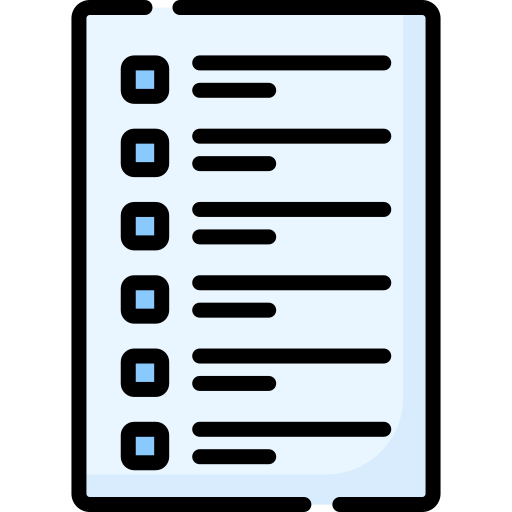
\includegraphics[width=1cm]{img/list.png}
                    
                    & 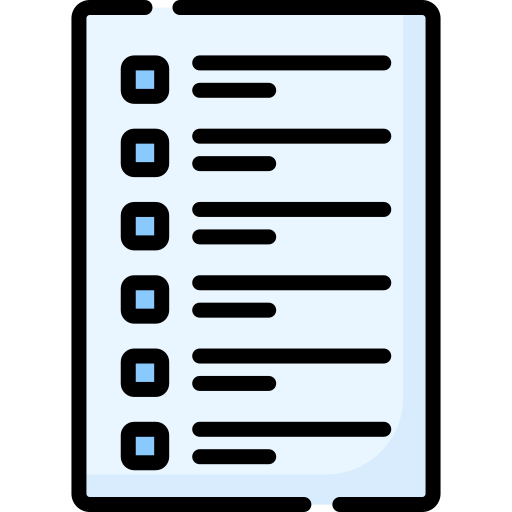
\includegraphics[width=1cm]{img/list.png}
                    & 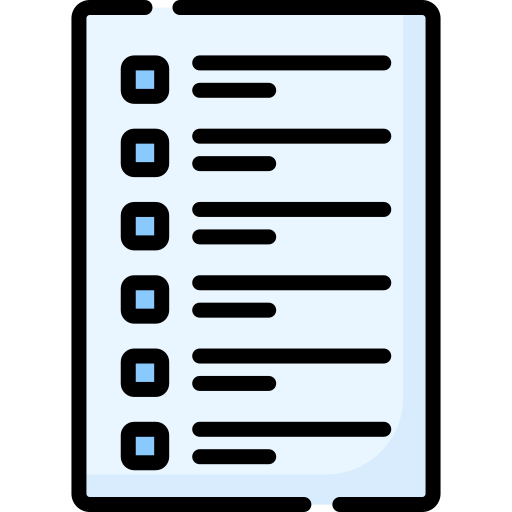
\includegraphics[width=1cm]{img/list.png}\\
    
                    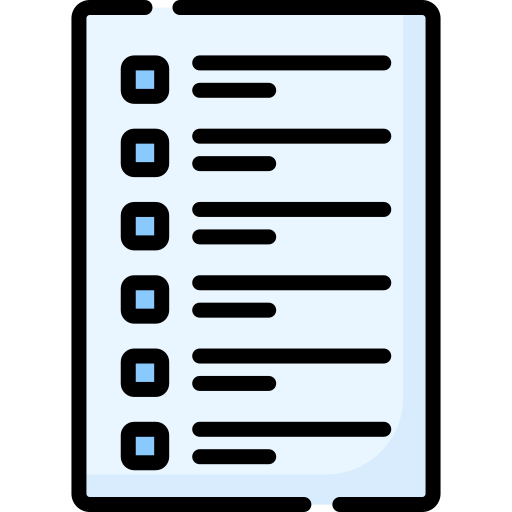
\includegraphics[width=1cm]{img/list.png}
                    & 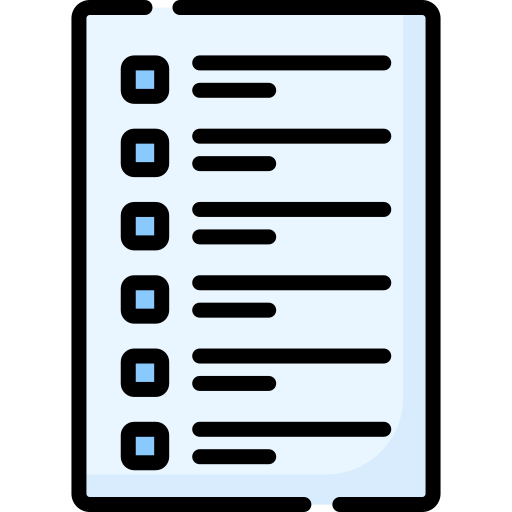
\includegraphics[width=1cm]{img/list.png}
                    & 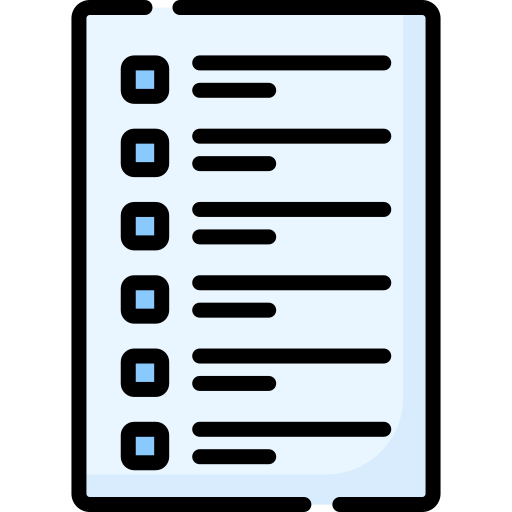
\includegraphics[width=1cm]{img/list.png}\\
    
                    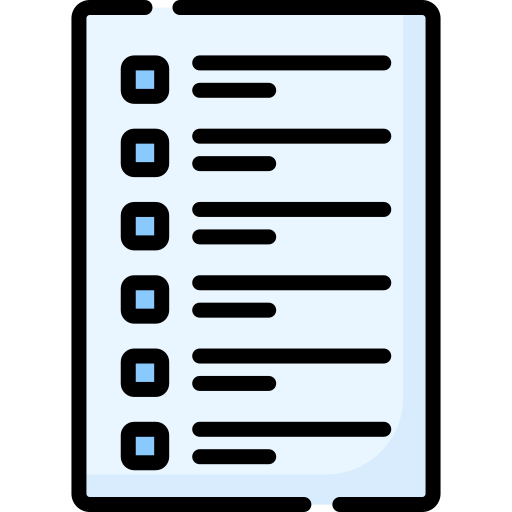
\includegraphics[width=1cm]{img/list.png}
                    & 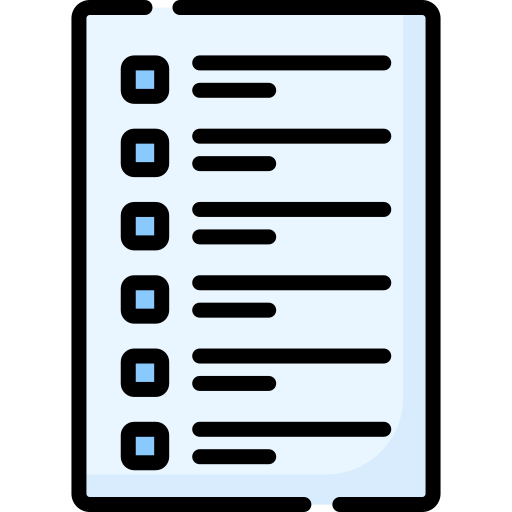
\includegraphics[width=1cm]{img/list.png}
                    & 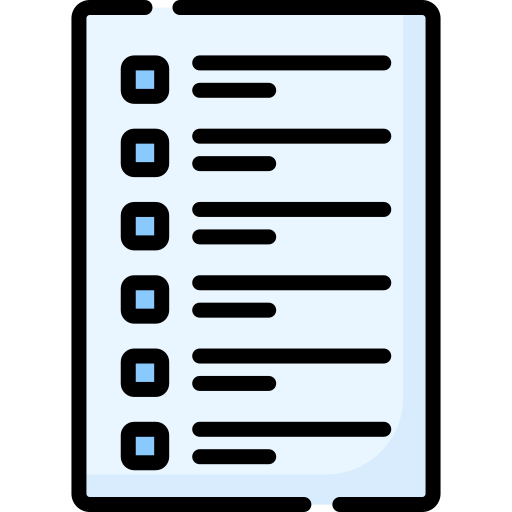
\includegraphics[width=1cm]{img/list.png}\\
    
    
                    ... & ... & ...\\
    
                    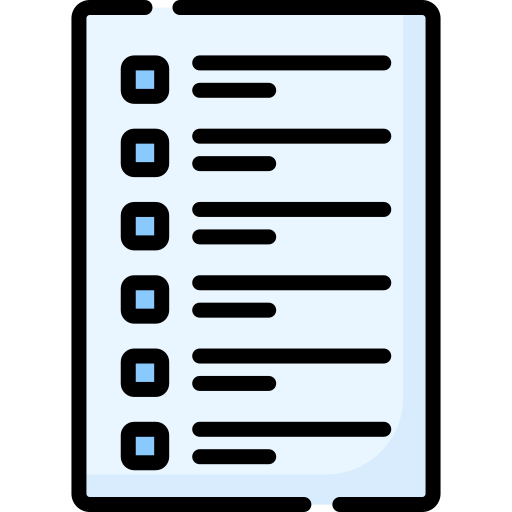
\includegraphics[width=1cm]{img/list.png}
                    & 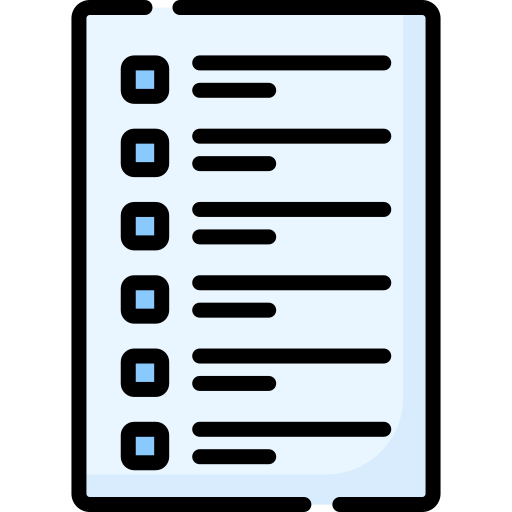
\includegraphics[width=1cm]{img/list.png}
                    & 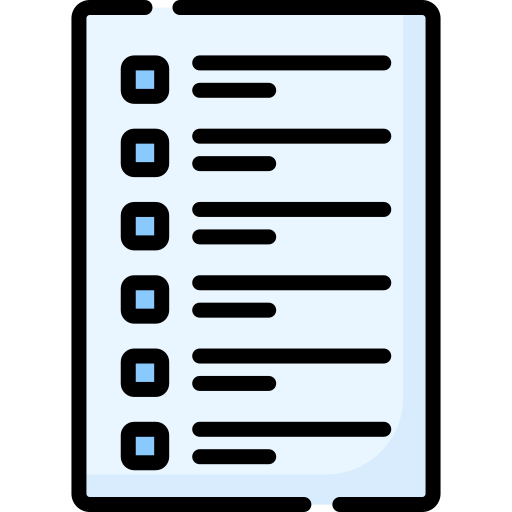
\includegraphics[width=1cm]{img/list.png}\\
    
                    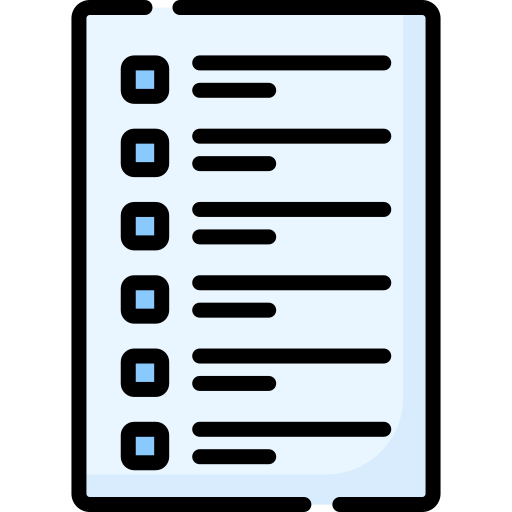
\includegraphics[width=1cm]{img/list.png}
                    & 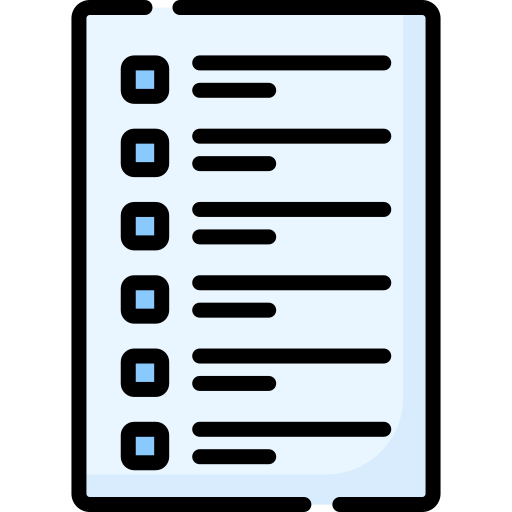
\includegraphics[width=1cm]{img/list.png}
                    & 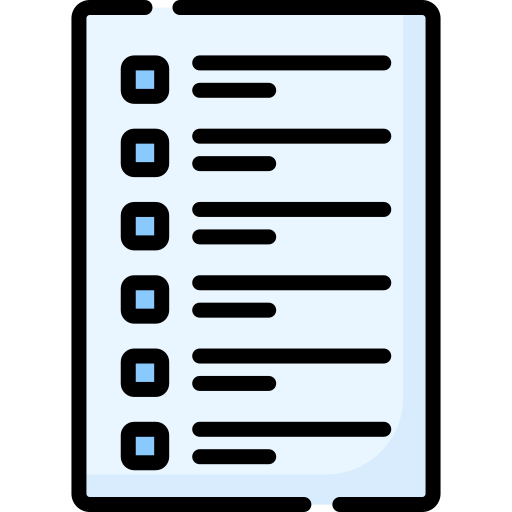
\includegraphics[width=1cm]{img/list.png}\\
    
                \end{tabular}
            \end{block}
            
    \end{column}

    


        \begin{column}{0.68\linewidth}
            \begin{block}{Caracter\'isticas}
                \begin{itemize}
                    \item Se crean nuevos ficheros a medida que se crean nuevos tipos de registros o se eliminan los ficheros.
                    \item Cada fichero se opera de forma independiente del resto de archivos en almacenamiento.
                \end{itemize}
                 
            \end{block}
            \begin{alertblock}<2->{Limitaciones}
                \begin{itemize}
                    \item<2-> Baja eficiencia
                    \item<3-> Gran redundancia de los datos
                    \item<4-> Pobre control sobre los datos
                    \item<5-> Capacidades inadecuadas de manipulaci\'on de datos
                \end{itemize}
            \end{alertblock}
        \end{column}

    \end{columns}

    \note<1>{@NOTE fue el 1er recurso digital para almacenar grandes vol\'umenes de datos}

    \note<1>{@NOTE por ``eliminar'' no solamente me refiero a borrar, sino tambi\'en a ignorar}

    \note<1>{@NOTE no hay manera de enlazar esos ficheros}

    \note<2>{@NOTE b\'usqueda secuencial}

    \note<3>{@NOTE debido a q no est\'an relacionados. Por qu\'e creen q esto sea una limitaci\'on? Esto lleva f\'acilmente a inconsistencias}

    \note<4>{@NOTE producto de la redundancia y la no relaci\'on entre los datos}

    \note<5>{@NOTE cada desarrollador deb\'ia implementar sus propias operaciones de manipulaci\'on de datos}
\end{frame}